\documentclass[11pt,preprint, authoryear]{elsarticle}

\usepackage{lmodern}
%%%% My spacing
\usepackage{setspace}
\setstretch{1.2}
\DeclareMathSizes{12}{14}{10}{10}

% Wrap around which gives all figures included the [H] command, or places it "here". This can be tedious to code in Rmarkdown.
\usepackage{float}
\let\origfigure\figure
\let\endorigfigure\endfigure
\renewenvironment{figure}[1][2] {
    \expandafter\origfigure\expandafter[H]
} {
    \endorigfigure
}

\let\origtable\table
\let\endorigtable\endtable
\renewenvironment{table}[1][2] {
    \expandafter\origtable\expandafter[H]
} {
    \endorigtable
}


\usepackage{ifxetex,ifluatex}
\usepackage{fixltx2e} % provides \textsubscript
\ifnum 0\ifxetex 1\fi\ifluatex 1\fi=0 % if pdftex
  \usepackage[T1]{fontenc}
  \usepackage[utf8]{inputenc}
\else % if luatex or xelatex
  \ifxetex
    \usepackage{mathspec}
    \usepackage{xltxtra,xunicode}
  \else
    \usepackage{fontspec}
  \fi
  \defaultfontfeatures{Mapping=tex-text,Scale=MatchLowercase}
  \newcommand{\euro}{€}
\fi

\usepackage{amssymb, amsmath, amsthm, amsfonts}

\def\bibsection{\section*{References}} %%% Make "References" appear before bibliography


\usepackage[round]{natbib}

\usepackage{longtable}
\usepackage[margin=2.3cm,bottom=2cm,top=2.5cm, includefoot]{geometry}
\usepackage{fancyhdr}
\usepackage[bottom, hang, flushmargin]{footmisc}
\usepackage{graphicx}
\numberwithin{equation}{section}
\numberwithin{figure}{section}
\numberwithin{table}{section}
\setlength{\parindent}{0cm}
\setlength{\parskip}{1.3ex plus 0.5ex minus 0.3ex}
\usepackage{textcomp}
\renewcommand{\headrulewidth}{0pt}

\usepackage{array}
\newcolumntype{x}[1]{>{\centering\arraybackslash\hspace{0pt}}p{#1}}

%%%%  Remove the "preprint submitted to" part. Don't worry about this either, it just looks better without it:
\makeatletter
\def\ps@pprintTitle{%
  \let\@oddhead\@empty
  \let\@evenhead\@empty
  \let\@oddfoot\@empty
  \let\@evenfoot\@oddfoot
}
\makeatother

 \def\tightlist{} % This allows for subbullets!

\usepackage{hyperref}
\hypersetup{breaklinks=true,
            bookmarks=true,
            colorlinks=true,
            citecolor=blue,
            urlcolor=blue,
            linkcolor=blue,
            pdfborder={0 0 0}}


% The following packages allow huxtable to work:
\usepackage{siunitx}
\usepackage{multirow}
\usepackage{hhline}
\usepackage{calc}
\usepackage{tabularx}
\usepackage{booktabs}
\usepackage{caption}


\newenvironment{columns}[1][]{}{}

\newenvironment{column}[1]{\begin{minipage}{#1}\ignorespaces}{%
\end{minipage}
\ifhmode\unskip\fi
\aftergroup\useignorespacesandallpars}

\def\useignorespacesandallpars#1\ignorespaces\fi{%
#1\fi\ignorespacesandallpars}

\makeatletter
\def\ignorespacesandallpars{%
  \@ifnextchar\par
    {\expandafter\ignorespacesandallpars\@gobble}%
    {}%
}
\makeatother

\newlength{\cslhangindent}
\setlength{\cslhangindent}{1.5em}
\newenvironment{CSLReferences}%
  {\setlength{\parindent}{0pt}%
  \everypar{\setlength{\hangindent}{\cslhangindent}}\ignorespaces}%
  {\par}


\urlstyle{same}  % don't use monospace font for urls
\setlength{\parindent}{0pt}
\setlength{\parskip}{6pt plus 2pt minus 1pt}
\setlength{\emergencystretch}{3em}  % prevent overfull lines
\setcounter{secnumdepth}{5}

%%% Use protect on footnotes to avoid problems with footnotes in titles
\let\rmarkdownfootnote\footnote%
\def\footnote{\protect\rmarkdownfootnote}
\IfFileExists{upquote.sty}{\usepackage{upquote}}{}

%%% Include extra packages specified by user

%%% Hard setting column skips for reports - this ensures greater consistency and control over the length settings in the document.
%% page layout
%% paragraphs
\setlength{\baselineskip}{12pt plus 0pt minus 0pt}
\setlength{\parskip}{12pt plus 0pt minus 0pt}
\setlength{\parindent}{0pt plus 0pt minus 0pt}
%% floats
\setlength{\floatsep}{12pt plus 0 pt minus 0pt}
\setlength{\textfloatsep}{20pt plus 0pt minus 0pt}
\setlength{\intextsep}{14pt plus 0pt minus 0pt}
\setlength{\dbltextfloatsep}{20pt plus 0pt minus 0pt}
\setlength{\dblfloatsep}{14pt plus 0pt minus 0pt}
%% maths
\setlength{\abovedisplayskip}{12pt plus 0pt minus 0pt}
\setlength{\belowdisplayskip}{12pt plus 0pt minus 0pt}
%% lists
\setlength{\topsep}{10pt plus 0pt minus 0pt}
\setlength{\partopsep}{3pt plus 0pt minus 0pt}
\setlength{\itemsep}{5pt plus 0pt minus 0pt}
\setlength{\labelsep}{8mm plus 0mm minus 0mm}
\setlength{\parsep}{\the\parskip}
\setlength{\listparindent}{\the\parindent}
%% verbatim
\setlength{\fboxsep}{5pt plus 0pt minus 0pt}



\begin{document}



\begin{frontmatter}  %

\title{How do oil price changes impact economic variables in the period
1990 to 2017: A Replication of the Cologni \& Manera paper}

% Set to FALSE if wanting to remove title (for submission)




\author[Add1]{Harriet Catherine Laing}
\ead{21617023@sun.ac.za}





\address[Add1]{Stellenbosch University, Stellenbosch, South Africa}



\vspace{1cm}





\vspace{0.5cm}

\end{frontmatter}



%________________________
% Header and Footers
%%%%%%%%%%%%%%%%%%%%%%%%%%%%%%%%%
\pagestyle{fancy}
\chead{}
\rhead{}
\lfoot{}
\rfoot{\footnotesize Page \thepage}
\lhead{}
%\rfoot{\footnotesize Page \thepage } % "e.g. Page 2"
\cfoot{}

%\setlength\headheight{30pt}
%%%%%%%%%%%%%%%%%%%%%%%%%%%%%%%%%
%________________________

\headsep 35pt % So that header does not go over title




\hypertarget{introduction}{%
\section{\texorpdfstring{Introduction
\label{Introduction}}{Introduction }}\label{introduction}}

To replicate the study by Cologni \& Manera to find the economic impact
of a rise in oil prices.

\hypertarget{background}{%
\section{Background}\label{background}}

\hypertarget{replication-methodology-results}{%
\section{Replication methodology \&
results}\label{replication-methodology-results}}

\hypertarget{step-1-find-the-data}{%
\section{Step 1: Find the data}\label{step-1-find-the-data}}

As per the paper, the data was sourced where possible from the IMF.
However, for the interest rate and exchange rate we sourced the data
from Board of Governors of the Federal Reserve System and for inflation
from the US Bureau of Labor Statistics. First, we want to use US data
and see if we can replicate the results in the study. We need to convert
all the data into quarterly. The time period available to reproduce the
results of the paper was constrained by the availability of world oil
price data: could only find from 1990, therefore had to limit to 1990
onwards. Similarly, restricted time period due to the data availability
of money. In the paper they used predominantly seasonally-adjusted data
but due to constraints on availability of data, for this replication I
used a combination of seasonally-adjusted and not seasonally-adjusted.

Interest Rate= Federal Funds Effective Rate, percent, not seasonally
adjusted, monthly Source: Board of Governors of the Federal Reserve
System Exchange Rate= Millions of Dollars, Not Seasonally Adjusted,
quarterly, source: Board of Governors of the Federal Reserve System
(2021) Inflation = Index 1982-1984=100, Seasonally Adjusted, monthly,
source U.S. Bureau of Labor Statistics Real GDP = Domestic Currency,
Seasonally Adjusted, quarterly, source IMF Monetary Aggregate = Dollars,
Seasonally Adjusted, monthly source: IMF World Oil Price = U.S. Dollars
per Barrel, Not Seasonally Adjusted, monthly, IMF. Need to do until 2017
because of monetary aggregate data constraints

The methodology that I applied in order to replicate the study, was to
first transform all of the quarterly series in logarithms except for the
interest rate. As in the paper, we run Augmented Dickey Fuller tests on
all the time series variables. Findings at the 1\% confidence interval
were that are all variables were non-stationary and were integrated of
order 1, except for the monetary aggregate which was found to be
integrated of order 2. The lags were selected according to the AIC
criteria, as done in the paper. The results in this replication differed
only from the paper regarding the integration order of inflation, which
was found to be integrated of order 1 by Cologni \& Manera. This
difference from the paper dictated that only the monetary aggregate be
transformed by subtracting inflation to become the real monetary
aggregate (by taking the difference between the logarithm of monetary
aggregate and the logarithm of inflation), and the transformation for
inflation was not followed. This is because for finding cointegrating
relationships, the time series variables must be integrated of order 1.

Resultant time series variables were as follows:

\begin{center}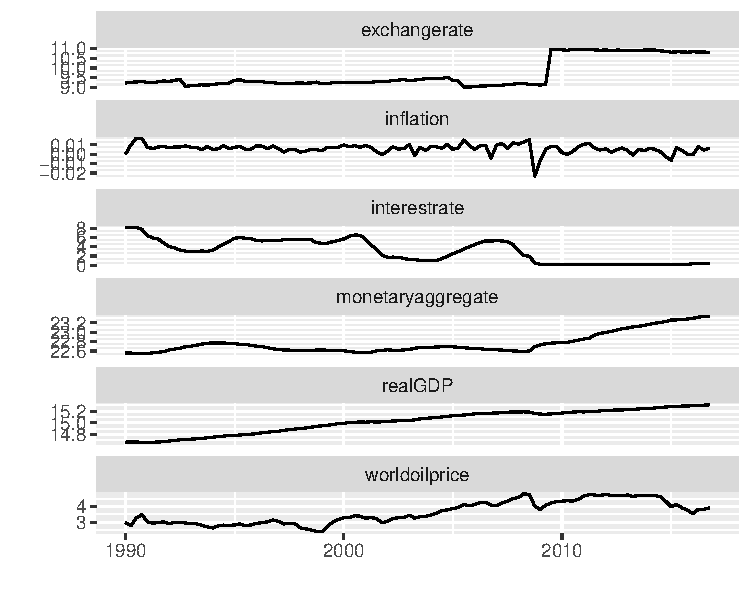
\includegraphics{README_files/figure-latex/unnamed-chunk-1-1} \end{center}

\begin{center}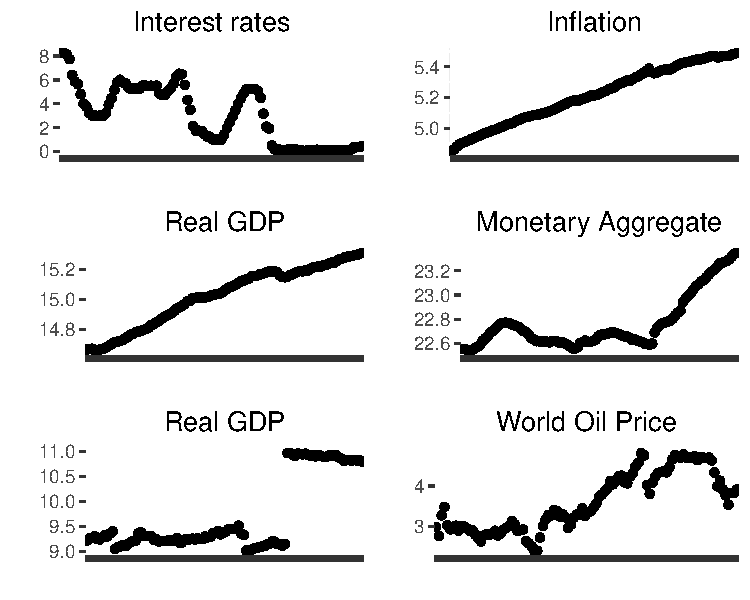
\includegraphics{README_files/figure-latex/unnamed-chunk-2-1} \end{center}

We then construct our VAR model by creating a matrix which includes the
time series variables included in Figure 1. We set the lag max to 4. The
VAR model was found to have 3 lags (4 - 1) when we used the AIC lag
selection criteria and accounted for a time trend, as is done in the
paper.

\begin{verbatim}
## AIC(n)  HQ(n)  SC(n) FPE(n) 
##      4      2      1      4
\end{verbatim}

Use AIC and find that lag should be 2 according to the paper, but we
find AIC suggests 4, so we use 3. As can be seen in Figure 1, there is
clearly a lot of persistence after the financial crisis. Exchange rates
for the US had a stark level increase around this water-shed event and
interest rates were set close to zero to try and stimulate the economy,
where they have remained fairly constant since this monetary policy
adjustment. Similarly, we can note real GDP has diminished since 2008.

Now we can see long-run trends in the time series variables, but wish to
now see if there exists any cointegrating relationships. We test this
using the Johansen test, namely the eigenvalue test and the trace test.
For the eigenvalue test, we find that we can reject the null hypothesis
of the number of cointegrating relationships equalling 3 or exceeding it
at the 5\% confidence interval where our critical value is smaller than
the test statistic. For the trace test, we find that we can reject the
null hypothesis when the relationships equal or exceed 2. Therefore,
because the rejection of the null hypothesis in the eigenvalue test is
incredibly marginal (25.71 critical value marginally larger than 25.54
test statistic), we conclude from our estimates that there is likely one
cointegrating relationship. This is the same result as is found for the
US in Cologni \& Manera.

We obtain the cointegrating vectors from the Johansen test and construct
a matrix is which each column is a cointegrating vector. Then we
multiply the VAR system by the cointegrating vector matrix to obtain the
error correction terms.

Let us set up the imposed restrictions in a matrix, known as B matrix in
the paper.

\begin{verbatim}
##       [,1] [,2] [,3] [,4] [,5] [,6]
## Brow1    1    1    0    1    0    0
## Brow2    0    1    1    1    1    1
## Brow3    0    0    1    1    1    1
## Brow4    0    0    0    1    1    1
## Brow5    0    0    0    0    1    1
## Brow6    0    0    0    0    0    1
\end{verbatim}

Let us see if we can impose the restrictions contained in the B matrix
onto the cointegrating vectors contained in the Et matrix.

\begin{verbatim}
##             [,1]        [,2]         [,3]         [,4]         [,5]
## [1,] -0.03485871  0.01603781  0.000000000  0.001526585  0.000000000
## [2,]  0.00000000 -0.03217102 -0.011618819 -0.000240614 -0.022636950
## [3,]  0.00000000  0.00000000  0.004480429 -0.032083484  0.016714331
## [4,]  0.00000000  0.00000000  0.000000000 -0.139231280 -0.012532633
## [5,]  0.00000000  0.00000000  0.000000000  0.000000000 -0.008558293
## [6,]  0.00000000  0.00000000  0.000000000  0.000000000  0.000000000
##               [,6]
## [1,]  0.000000e+00
## [2,] -5.406431e-03
## [3,] -5.789421e-03
## [4,] -8.313818e-03
## [5,] -8.248844e-05
## [6,]  9.414487e-03
\end{verbatim}

\hypertarget{set-up-vecm}{%
\section{Set up VECM}\label{set-up-vecm}}

\begin{verbatim}
## #############
## ###Model VECM 
## #############
## Full sample size: 108    End sample size: 104
## Number of variables: 6   Number of estimated slope parameters 120
## AIC -3198.134    BIC -2867.585   SSR 75.25772
## Cointegrating vector (estimated by ML):
##    MonetaryAggregate InterestRate  RealGDP  Inflation ExchangeRate
## r1                 1    -0.134276 4.787817 -0.0522194     0.615354
##    WorldOilPrice
## r1     0.4247612
## 
## 
##                            ECT                 Intercept          
## Equation MonetaryAggregate 0.0126(0.0045)**    -1.1623(0.4105)**  
## Equation InterestRate      -0.0200(0.1043)     1.9540(9.5628)     
## Equation RealGDP           0.0005(0.0020)      -0.0411(0.1876)    
## Equation Inflation         -0.0750(0.3299)     8.4465(30.2481)    
## Equation ExchangeRate      -0.1963(0.0391)***  18.3351(3.5838)*** 
## Equation WorldOilPrice     -0.0645(0.0542)     6.0297(4.9693)     
##                            MonetaryAggregate -1 InterestRate -1    
## Equation MonetaryAggregate 0.4105(0.1324)**     0.0031(0.0046)     
## Equation InterestRate      -0.3107(3.0852)      0.5676(0.1068)***  
## Equation RealGDP           -0.0478(0.0605)      -0.0022(0.0021)    
## Equation Inflation         -0.1479(9.7587)      -0.8517(0.3377)*   
## Equation ExchangeRate      -0.0068(1.1562)      0.0353(0.0400)     
## Equation WorldOilPrice     -0.0068(1.6032)      -0.0309(0.0555)    
##                            RealGDP -1           Inflation -1       
## Equation MonetaryAggregate -0.3634(0.2590)      0.0094(0.0022)***  
## Equation InterestRate      8.9686(6.0343)       -0.1328(0.0503)**  
## Equation RealGDP           0.3067(0.1184)*      -0.0007(0.0010)    
## Equation Inflation         25.2237(19.0871)     -0.3050(0.1591).   
## Equation ExchangeRate      -0.2586(2.2614)      -0.0372(0.0189).   
## Equation WorldOilPrice     5.6317(3.1357).      -0.0643(0.0261)*   
##                            ExchangeRate -1     WorldOilPrice -1   
## Equation MonetaryAggregate -0.0031(0.0073)     -0.0391(0.0131)**  
## Equation InterestRate      -0.0114(0.1698)     0.4794(0.3046)     
## Equation RealGDP           0.0026(0.0033)      -0.0013(0.0060)    
## Equation Inflation         0.1635(0.5372)      4.0925(0.9635)***  
## Equation ExchangeRate      -0.2607(0.0636)***  0.3036(0.1142)**   
## Equation WorldOilPrice     0.0616(0.0882)      0.4672(0.1583)**   
##                            MonetaryAggregate -2 InterestRate -2    
## Equation MonetaryAggregate -0.0357(0.1367)      -0.0010(0.0054)    
## Equation InterestRate      4.6836(3.1852)       0.0479(0.1247)     
## Equation RealGDP           0.0919(0.0625)       0.0021(0.0024)     
## Equation Inflation         4.6173(10.0751)      0.1513(0.3946)     
## Equation ExchangeRate      0.7482(1.1937)       0.0708(0.0468)     
## Equation WorldOilPrice     2.2347(1.6552)       -0.0113(0.0648)    
##                            RealGDP -2           Inflation -2       
## Equation MonetaryAggregate -0.5758(0.2612)*     0.0015(0.0022)     
## Equation InterestRate      -0.5452(6.0847)      0.0186(0.0511)     
## Equation RealGDP           0.2504(0.1194)*      -0.0009(0.0010)    
## Equation Inflation         -8.8860(19.2466)     -0.1707(0.1615)    
## Equation ExchangeRate      -5.6094(2.2803)*     -0.0100(0.0191)    
## Equation WorldOilPrice     0.4852(3.1619)       -0.0251(0.0265)    
##                            ExchangeRate -2     WorldOilPrice -2   
## Equation MonetaryAggregate -0.0013(0.0068)     -0.0075(0.0133)    
## Equation InterestRate      -0.1535(0.1591)     -0.3310(0.3089)    
## Equation RealGDP           -0.0028(0.0031)     0.0035(0.0061)     
## Equation Inflation         -0.7990(0.5032)     0.9032(0.9770)     
## Equation ExchangeRate      -0.0974(0.0596)     -0.0140(0.1157)    
## Equation WorldOilPrice     -0.0530(0.0827)     0.0298(0.1605)     
##                            MonetaryAggregate -3 InterestRate -3    
## Equation MonetaryAggregate 0.0399(0.1264)       -0.0120(0.0045)**  
## Equation InterestRate      1.5625(2.9449)       0.0465(0.1056)     
## Equation RealGDP           -0.0549(0.0578)      0.0009(0.0021)     
## Equation Inflation         -0.9284(9.3150)      0.9919(0.3339)**   
## Equation ExchangeRate      2.9212(1.1036)**     -0.0599(0.0396)    
## Equation WorldOilPrice     -0.6155(1.5303)      0.0691(0.0549)     
##                            RealGDP -3           Inflation -3       
## Equation MonetaryAggregate 0.3512(0.2735)       0.0037(0.0021).    
## Equation InterestRate      5.8409(6.3702)       -0.1417(0.0488)**  
## Equation RealGDP           -0.0610(0.1250)      -0.0016(0.0010)    
## Equation Inflation         -9.7967(20.1495)     -0.0537(0.1543)    
## Equation ExchangeRate      -10.5904(2.3873)***  -0.1229(0.0183)*** 
## Equation WorldOilPrice     -1.3140(3.3102)      -0.0394(0.0253)    
##                            ExchangeRate -3     WorldOilPrice -3   
## Equation MonetaryAggregate 0.0004(0.0068)      -0.0189(0.0127)    
## Equation InterestRate      -0.0609(0.1588)     1.2460(0.2968)***  
## Equation RealGDP           0.0013(0.0031)      0.0060(0.0058)     
## Equation Inflation         -0.6361(0.5022)     0.3802(0.9388)     
## Equation ExchangeRate      0.0260(0.0595)      0.3845(0.1112)***  
## Equation WorldOilPrice     0.0156(0.0825)      0.2993(0.1542).
\end{verbatim}

Then test for white noise residuals.

\hypertarget{step-3-augemented-dickey-fuller-tests}{%
\section{Step 3: Augemented Dickey-Fuller
tests}\label{step-3-augemented-dickey-fuller-tests}}

The null-hypothesis of an Augmented Dickey-Fuller test is that the
series has a unit-root. We ask, is the estimated critical value small
enough to reject the null-hypothesis? If yes, we cannot reject the null
hypothesis, therefore, the series may be non-stationary.

In this section, we find that the interest rate is stationary, change in
inflation is stationary, detrended real GDP is still not stationary,
detrended monetary aggregate is still non-stationary and world oil price
is non stationary.

\hypertarget{augmented-dickey-fuller-tests}{%
\section{Augmented Dickey Fuller
tests}\label{augmented-dickey-fuller-tests}}

\begin{verbatim}
## 
## ############################################### 
## # Augmented Dickey-Fuller Test Unit Root Test # 
## ############################################### 
## 
## Test regression none 
## 
## 
## Call:
## lm(formula = z.diff ~ z.lag.1 - 1 + z.diff.lag)
## 
## Residuals:
##      Min       1Q   Median       3Q      Max 
## -1.30124 -0.04024  0.03284  0.19765  0.64002 
## 
## Coefficients:
##             Estimate Std. Error t value Pr(>|t|)    
## z.lag.1    -0.017754   0.007925  -2.240   0.0272 *  
## z.diff.lag  0.665828   0.070243   9.479 9.82e-16 ***
## ---
## Signif. codes:  0 '***' 0.001 '**' 0.01 '*' 0.05 '.' 0.1 ' ' 1
## 
## Residual standard error: 0.3117 on 104 degrees of freedom
## Multiple R-squared:  0.4962, Adjusted R-squared:  0.4865 
## F-statistic: 51.22 on 2 and 104 DF,  p-value: 3.283e-16
## 
## 
## Value of test-statistic is: -2.2403 
## 
## Critical values for test statistics: 
##       1pct  5pct 10pct
## tau1 -2.58 -1.95 -1.62
\end{verbatim}

\begin{verbatim}
## 
## ############################################### 
## # Augmented Dickey-Fuller Test Unit Root Test # 
## ############################################### 
## 
## Test regression none 
## 
## 
## Call:
## lm(formula = z.diff ~ z.lag.1 - 1 + z.diff.lag)
## 
## Residuals:
##      Min       1Q   Median       3Q      Max 
## -1.26565 -0.04976  0.00946  0.14002  0.64079 
## 
## Coefficients:
##            Estimate Std. Error t value Pr(>|t|)    
## z.lag.1    -0.29184    0.07777  -3.753  0.00029 ***
## z.diff.lag -0.06765    0.09829  -0.688  0.49278    
## ---
## Signif. codes:  0 '***' 0.001 '**' 0.01 '*' 0.05 '.' 0.1 ' ' 1
## 
## Residual standard error: 0.3199 on 103 degrees of freedom
## Multiple R-squared:  0.1604, Adjusted R-squared:  0.1441 
## F-statistic:  9.84 on 2 and 103 DF,  p-value: 0.0001228
## 
## 
## Value of test-statistic is: -3.7526 
## 
## Critical values for test statistics: 
##       1pct  5pct 10pct
## tau1 -2.58 -1.95 -1.62
\end{verbatim}

\begin{verbatim}
## 
## ############################################### 
## # Augmented Dickey-Fuller Test Unit Root Test # 
## ############################################### 
## 
## Test regression none 
## 
## 
## Call:
## lm(formula = z.diff ~ z.lag.1 - 1 + z.diff.lag)
## 
## Residuals:
##       Min        1Q    Median        3Q       Max 
## -0.031918 -0.001413  0.000394  0.002783  0.010390 
## 
## Coefficients:
##             Estimate Std. Error t value Pr(>|t|)    
## z.lag.1    0.0007928  0.0001390   5.703 1.11e-07 ***
## z.diff.lag 0.2926254  0.0935172   3.129  0.00228 ** 
## ---
## Signif. codes:  0 '***' 0.001 '**' 0.01 '*' 0.05 '.' 0.1 ' ' 1
## 
## Residual standard error: 0.004852 on 104 degrees of freedom
## Multiple R-squared:  0.6129, Adjusted R-squared:  0.6054 
## F-statistic: 82.32 on 2 and 104 DF,  p-value: < 2.2e-16
## 
## 
## Value of test-statistic is: 5.7029 
## 
## Critical values for test statistics: 
##       1pct  5pct 10pct
## tau1 -2.58 -1.95 -1.62
\end{verbatim}

\begin{verbatim}
## 
## ############################################### 
## # Augmented Dickey-Fuller Test Unit Root Test # 
## ############################################### 
## 
## Test regression none 
## 
## 
## Call:
## lm(formula = z.diff ~ z.lag.1 - 1 + z.diff.lag)
## 
## Residuals:
##       Min        1Q    Median        3Q       Max 
## -0.033954 -0.000482  0.002075  0.004001  0.012994 
## 
## Coefficients:
##            Estimate Std. Error t value Pr(>|t|)    
## z.lag.1    -0.26980    0.07387  -3.652  0.00041 ***
## z.diff.lag -0.16294    0.09511  -1.713  0.08968 .  
## ---
## Signif. codes:  0 '***' 0.001 '**' 0.01 '*' 0.05 '.' 0.1 ' ' 1
## 
## Residual standard error: 0.005415 on 103 degrees of freedom
## Multiple R-squared:  0.1927, Adjusted R-squared:  0.177 
## F-statistic: 12.29 on 2 and 103 DF,  p-value: 1.628e-05
## 
## 
## Value of test-statistic is: -3.6524 
## 
## Critical values for test statistics: 
##       1pct  5pct 10pct
## tau1 -2.58 -1.95 -1.62
\end{verbatim}

Real GDP

\begin{verbatim}
## 
## ############################################### 
## # Augmented Dickey-Fuller Test Unit Root Test # 
## ############################################### 
## 
## Test regression none 
## 
## 
## Call:
## lm(formula = z.diff ~ z.lag.1 - 1 + z.diff.lag)
## 
## Residuals:
##        Min         1Q     Median         3Q        Max 
## -0.0234977 -0.0030666  0.0004404  0.0032845  0.0130056 
## 
## Coefficients:
##             Estimate Std. Error t value Pr(>|t|)    
## z.lag.1    2.365e-04  5.087e-05   4.649 9.84e-06 ***
## z.diff.lag 4.100e-01  8.943e-02   4.585 1.27e-05 ***
## ---
## Signif. codes:  0 '***' 0.001 '**' 0.01 '*' 0.05 '.' 0.1 ' ' 1
## 
## Residual standard error: 0.005598 on 104 degrees of freedom
## Multiple R-squared:  0.5797, Adjusted R-squared:  0.5716 
## F-statistic: 71.72 on 2 and 104 DF,  p-value: < 2.2e-16
## 
## 
## Value of test-statistic is: 4.6489 
## 
## Critical values for test statistics: 
##       1pct  5pct 10pct
## tau1 -2.58 -1.95 -1.62
\end{verbatim}

\begin{verbatim}
## 
## ############################################### 
## # Augmented Dickey-Fuller Test Unit Root Test # 
## ############################################### 
## 
## Test regression none 
## 
## 
## Call:
## lm(formula = z.diff ~ z.lag.1 - 1 + z.diff.lag)
## 
## Residuals:
##       Min        1Q    Median        3Q       Max 
## -0.021479 -0.002183  0.001511  0.004429  0.013011 
## 
## Coefficients:
##            Estimate Std. Error t value Pr(>|t|)    
## z.lag.1    -0.19720    0.07196  -2.740  0.00724 ** 
## z.diff.lag -0.33194    0.09306  -3.567  0.00055 ***
## ---
## Signif. codes:  0 '***' 0.001 '**' 0.01 '*' 0.05 '.' 0.1 ' ' 1
## 
## Residual standard error: 0.00583 on 103 degrees of freedom
## Multiple R-squared:  0.2414, Adjusted R-squared:  0.2267 
## F-statistic: 16.39 on 2 and 103 DF,  p-value: 6.62e-07
## 
## 
## Value of test-statistic is: -2.7403 
## 
## Critical values for test statistics: 
##       1pct  5pct 10pct
## tau1 -2.58 -1.95 -1.62
\end{verbatim}

Monetary Aggregates

\begin{verbatim}
## 
## ############################################### 
## # Augmented Dickey-Fuller Test Unit Root Test # 
## ############################################### 
## 
## Test regression none 
## 
## 
## Call:
## lm(formula = z.diff ~ z.lag.1 - 1 + z.diff.lag)
## 
## Residuals:
##       Min        1Q    Median        3Q       Max 
## -0.024123 -0.007572 -0.000144  0.005791  0.052443 
## 
## Coefficients:
##             Estimate Std. Error t value Pr(>|t|)    
## z.lag.1    0.0001535  0.0000529   2.902  0.00453 ** 
## z.diff.lag 0.6811085  0.0718457   9.480 9.76e-16 ***
## ---
## Signif. codes:  0 '***' 0.001 '**' 0.01 '*' 0.05 '.' 0.1 ' ' 1
## 
## Residual standard error: 0.01155 on 104 degrees of freedom
## Multiple R-squared:  0.6921, Adjusted R-squared:  0.6862 
## F-statistic: 116.9 on 2 and 104 DF,  p-value: < 2.2e-16
## 
## 
## Value of test-statistic is: 2.902 
## 
## Critical values for test statistics: 
##       1pct  5pct 10pct
## tau1 -2.58 -1.95 -1.62
\end{verbatim}

\begin{verbatim}
## 
## ############################################### 
## # Augmented Dickey-Fuller Test Unit Root Test # 
## ############################################### 
## 
## Test regression none 
## 
## 
## Call:
## lm(formula = z.diff ~ z.lag.1 - 1 + z.diff.lag)
## 
## Residuals:
##       Min        1Q    Median        3Q       Max 
## -0.021316 -0.005213  0.000844  0.007164  0.051563 
## 
## Coefficients:
##            Estimate Std. Error t value Pr(>|t|)  
## z.lag.1    -0.13784    0.05814  -2.371   0.0196 *
## z.diff.lag -0.24266    0.09651  -2.514   0.0135 *
## ---
## Signif. codes:  0 '***' 0.001 '**' 0.01 '*' 0.05 '.' 0.1 ' ' 1
## 
## Residual standard error: 0.0117 on 103 degrees of freedom
## Multiple R-squared:  0.1441, Adjusted R-squared:  0.1275 
## F-statistic: 8.672 on 2 and 103 DF,  p-value: 0.0003305
## 
## 
## Value of test-statistic is: -2.3707 
## 
## Critical values for test statistics: 
##       1pct  5pct 10pct
## tau1 -2.58 -1.95 -1.62
\end{verbatim}

Exchange Rate

\begin{verbatim}
## 
## ############################################### 
## # Augmented Dickey-Fuller Test Unit Root Test # 
## ############################################### 
## 
## Test regression none 
## 
## 
## Call:
## lm(formula = z.diff ~ z.lag.1 - 1 + z.diff.lag)
## 
## Residuals:
##      Min       1Q   Median       3Q      Max 
## -0.36660 -0.02652 -0.00900  0.01104  1.80232 
## 
## Coefficients:
##            Estimate Std. Error t value Pr(>|t|)
## z.lag.1    0.001348   0.001877   0.718    0.474
## z.diff.lag 0.005283   0.098225   0.054    0.957
## 
## Residual standard error: 0.187 on 104 degrees of freedom
## Multiple R-squared:  0.005078,   Adjusted R-squared:  -0.01406 
## F-statistic: 0.2654 on 2 and 104 DF,  p-value: 0.7674
## 
## 
## Value of test-statistic is: 0.7184 
## 
## Critical values for test statistics: 
##       1pct  5pct 10pct
## tau1 -2.58 -1.95 -1.62
\end{verbatim}

\begin{verbatim}
## 
## ############################################### 
## # Augmented Dickey-Fuller Test Unit Root Test # 
## ############################################### 
## 
## Test regression none 
## 
## 
## Call:
## lm(formula = z.diff ~ z.lag.1 - 1 + z.diff.lag)
## 
## Residuals:
##      Min       1Q   Median       3Q      Max 
## -0.35260 -0.01246  0.00443  0.02440  1.81361 
## 
## Coefficients:
##            Estimate Std. Error t value Pr(>|t|)    
## z.lag.1    -1.01592    0.13846  -7.338 5.18e-11 ***
## z.diff.lag  0.02795    0.09848   0.284    0.777    
## ---
## Signif. codes:  0 '***' 0.001 '**' 0.01 '*' 0.05 '.' 0.1 ' ' 1
## 
## Residual standard error: 0.1883 on 103 degrees of freedom
## Multiple R-squared:  0.4945, Adjusted R-squared:  0.4847 
## F-statistic: 50.38 on 2 and 103 DF,  p-value: 5.501e-16
## 
## 
## Value of test-statistic is: -7.3375 
## 
## Critical values for test statistics: 
##       1pct  5pct 10pct
## tau1 -2.58 -1.95 -1.62
\end{verbatim}

World Oil Price

\begin{verbatim}
## 
## ############################################### 
## # Augmented Dickey-Fuller Test Unit Root Test # 
## ############################################### 
## 
## Test regression none 
## 
## 
## Call:
## lm(formula = z.diff ~ z.lag.1 - 1 + z.diff.lag)
## 
## Residuals:
##      Min       1Q   Median       3Q      Max 
## -0.72572 -0.06453  0.01614  0.08600  0.53844 
## 
## Coefficients:
##            Estimate Std. Error t value Pr(>|t|)  
## z.lag.1    0.001240   0.004215   0.294    0.769  
## z.diff.lag 0.160192   0.096223   1.665    0.099 .
## ---
## Signif. codes:  0 '***' 0.001 '**' 0.01 '*' 0.05 '.' 0.1 ' ' 1
## 
## Residual standard error: 0.1595 on 104 degrees of freedom
## Multiple R-squared:  0.02747,    Adjusted R-squared:  0.008763 
## F-statistic: 1.469 on 2 and 104 DF,  p-value: 0.235
## 
## 
## Value of test-statistic is: 0.2942 
## 
## Critical values for test statistics: 
##       1pct  5pct 10pct
## tau1 -2.58 -1.95 -1.62
\end{verbatim}

\hypertarget{set-up-the-var-model}{%
\section{Set up the VAR model}\label{set-up-the-var-model}}

\hypertarget{build-var-model}{%
\section{Build VAR model}\label{build-var-model}}

\begin{verbatim}
## 
## VAR Estimation Results:
## ========================= 
## Endogenous variables: MonetaryAggregate, InterestRate, RealGDP, Inflation, ExchangeRate, WorldOilPrice 
## Deterministic variables: trend 
## Sample size: 105 
## Log Likelihood: 800.372 
## Roots of the characteristic polynomial:
## 1.001 0.9865 0.9865 0.9096 0.9096 0.8717 0.8717 0.6162 0.5794 0.5794 0.4751 0.4751 0.4373 0.4373 0.4058 0.4058 0.3981 0.3981
## Call:
## VAR(y = groupedVAR, p = 3, type = "trend", exogen = NULL)
## 
## 
## Estimation results for equation MonetaryAggregate: 
## ================================================== 
## MonetaryAggregate = MonetaryAggregate.l1 + InterestRate.l1 + RealGDP.l1 + Inflation.l1 + ExchangeRate.l1 + WorldOilPrice.l1 + MonetaryAggregate.l2 + InterestRate.l2 + RealGDP.l2 + Inflation.l2 + ExchangeRate.l2 + WorldOilPrice.l2 + MonetaryAggregate.l3 + InterestRate.l3 + RealGDP.l3 + Inflation.l3 + ExchangeRate.l3 + WorldOilPrice.l3 + trend 
## 
##                        Estimate Std. Error t value Pr(>|t|)    
## MonetaryAggregate.l1  1.3047772  0.1271001  10.266  < 2e-16 ***
## InterestRate.l1      -0.0010960  0.0047783  -0.229 0.819120    
## RealGDP.l1           -0.3187494  0.2467876  -1.292 0.199958    
## Inflation.l1          0.0087185  0.0021686   4.020 0.000124 ***
## ExchangeRate.l1      -0.0021688  0.0069313  -0.313 0.755113    
## WorldOilPrice.l1     -0.0343555  0.0122044  -2.815 0.006046 ** 
## MonetaryAggregate.l2 -0.3088679  0.2076664  -1.487 0.140586    
## InterestRate.l2      -0.0057323  0.0080447  -0.713 0.478048    
## RealGDP.l2           -0.0476563  0.3758990  -0.127 0.899411    
## Inflation.l2         -0.0051665  0.0030158  -1.713 0.090295 .  
## ExchangeRate.l2       0.0003534  0.0089754   0.039 0.968680    
## WorldOilPrice.l2      0.0237594  0.0164007   1.449 0.151062    
## MonetaryAggregate.l3 -0.0215402  0.1251202  -0.172 0.863719    
## InterestRate.l3       0.0037798  0.0045677   0.827 0.410245    
## RealGDP.l3            0.3787652  0.2520508   1.503 0.136571    
## Inflation.l3         -0.0008038  0.0021201  -0.379 0.705528    
## ExchangeRate.l3       0.0134310  0.0069299   1.938 0.055890 .  
## WorldOilPrice.l3     -0.0044031  0.0123397  -0.357 0.722095    
## trend                -0.0029500  0.0011267  -2.618 0.010439 *  
## ---
## Signif. codes:  0 '***' 0.001 '**' 0.01 '*' 0.05 '.' 0.1 ' ' 1
## 
## 
## Residual standard error: 0.01181 on 86 degrees of freedom
## Multiple R-Squared:     1,   Adjusted R-squared:     1 
## F-statistic: 2.055e+07 on 19 and 86 DF,  p-value: < 2.2e-16 
## 
## 
## Estimation results for equation InterestRate: 
## ============================================= 
## InterestRate = MonetaryAggregate.l1 + InterestRate.l1 + RealGDP.l1 + Inflation.l1 + ExchangeRate.l1 + WorldOilPrice.l1 + MonetaryAggregate.l2 + InterestRate.l2 + RealGDP.l2 + Inflation.l2 + ExchangeRate.l2 + WorldOilPrice.l2 + MonetaryAggregate.l3 + InterestRate.l3 + RealGDP.l3 + Inflation.l3 + ExchangeRate.l3 + WorldOilPrice.l3 + trend 
## 
##                        Estimate Std. Error t value Pr(>|t|)    
## MonetaryAggregate.l1  -1.952221   3.084476  -0.633   0.5285    
## InterestRate.l1        1.375258   0.115959  11.860   <2e-16 ***
## RealGDP.l1            14.290127   5.989063   2.386   0.0192 *  
## Inflation.l1          -0.083859   0.052628  -1.593   0.1147    
## ExchangeRate.l1       -0.163684   0.168210  -0.973   0.3332    
## WorldOilPrice.l1       0.140811   0.296178   0.475   0.6357    
## MonetaryAggregate.l2   3.003978   5.039666   0.596   0.5527    
## InterestRate.l2       -0.210108   0.195229  -1.076   0.2848    
## RealGDP.l2           -19.042812   9.122352  -2.087   0.0398 *  
## Inflation.l2           0.117266   0.073189   1.602   0.1128    
## ExchangeRate.l2        0.008949   0.217816   0.041   0.9673    
## WorldOilPrice.l2      -0.516657   0.398013  -1.298   0.1977    
## MonetaryAggregate.l3  -0.875961   3.036428  -0.288   0.7737    
## InterestRate.l3       -0.267204   0.110850  -2.410   0.0181 *  
## RealGDP.l3             4.714602   6.116792   0.771   0.4430    
## Inflation.l3          -0.045978   0.051451  -0.894   0.3740    
## ExchangeRate.l3       -0.001112   0.168175  -0.007   0.9947    
## WorldOilPrice.l3       0.415155   0.299460   1.386   0.1692    
## trend                  0.010115   0.027342   0.370   0.7123    
## ---
## Signif. codes:  0 '***' 0.001 '**' 0.01 '*' 0.05 '.' 0.1 ' ' 1
## 
## 
## Residual standard error: 0.2866 on 86 degrees of freedom
## Multiple R-Squared: 0.9951,  Adjusted R-squared: 0.994 
## F-statistic: 919.1 on 19 and 86 DF,  p-value: < 2.2e-16 
## 
## 
## Estimation results for equation RealGDP: 
## ======================================== 
## RealGDP = MonetaryAggregate.l1 + InterestRate.l1 + RealGDP.l1 + Inflation.l1 + ExchangeRate.l1 + WorldOilPrice.l1 + MonetaryAggregate.l2 + InterestRate.l2 + RealGDP.l2 + Inflation.l2 + ExchangeRate.l2 + WorldOilPrice.l2 + MonetaryAggregate.l3 + InterestRate.l3 + RealGDP.l3 + Inflation.l3 + ExchangeRate.l3 + WorldOilPrice.l3 + trend 
## 
##                        Estimate Std. Error t value Pr(>|t|)    
## MonetaryAggregate.l1 -0.0383785  0.0575594  -0.667    0.507    
## InterestRate.l1      -0.0018227  0.0021639  -0.842    0.402    
## RealGDP.l1            1.2456502  0.1117619  11.146   <2e-16 ***
## Inflation.l1          0.0002404  0.0009821   0.245    0.807    
## ExchangeRate.l1       0.0039487  0.0031390   1.258    0.212    
## WorldOilPrice.l1     -0.0087332  0.0055270  -1.580    0.118    
## MonetaryAggregate.l2  0.1079090  0.0940452   1.147    0.254    
## InterestRate.l2       0.0047055  0.0036432   1.292    0.200    
## RealGDP.l2           -0.0945479  0.1702322  -0.555    0.580    
## Inflation.l2         -0.0012468  0.0013658  -0.913    0.364    
## ExchangeRate.l2      -0.0048538  0.0040647  -1.194    0.236    
## WorldOilPrice.l2      0.0108246  0.0074273   1.457    0.149    
## MonetaryAggregate.l3 -0.0707778  0.0566628  -1.249    0.215    
## InterestRate.l3      -0.0032253  0.0020686  -1.559    0.123    
## RealGDP.l3           -0.1463459  0.1141455  -1.282    0.203    
## Inflation.l3          0.0006937  0.0009601   0.723    0.472    
## ExchangeRate.l3       0.0021952  0.0031383   0.699    0.486    
## WorldOilPrice.l3     -0.0042240  0.0055882  -0.756    0.452    
## trend                 0.0002802  0.0005102   0.549    0.584    
## ---
## Signif. codes:  0 '***' 0.001 '**' 0.01 '*' 0.05 '.' 0.1 ' ' 1
## 
## 
## Residual standard error: 0.005348 on 86 degrees of freedom
## Multiple R-Squared:     1,   Adjusted R-squared:     1 
## F-statistic: 4.367e+07 on 19 and 86 DF,  p-value: < 2.2e-16 
## 
## 
## Estimation results for equation Inflation: 
## ========================================== 
## Inflation = MonetaryAggregate.l1 + InterestRate.l1 + RealGDP.l1 + Inflation.l1 + ExchangeRate.l1 + WorldOilPrice.l1 + MonetaryAggregate.l2 + InterestRate.l2 + RealGDP.l2 + Inflation.l2 + ExchangeRate.l2 + WorldOilPrice.l2 + MonetaryAggregate.l3 + InterestRate.l3 + RealGDP.l3 + Inflation.l3 + ExchangeRate.l3 + WorldOilPrice.l3 + trend 
## 
##                       Estimate Std. Error t value Pr(>|t|)    
## MonetaryAggregate.l1   3.60914    9.42515   0.383 0.702719    
## InterestRate.l1       -0.63442    0.35433  -1.790 0.076898 .  
## RealGDP.l1            35.59225   18.30062   1.945 0.055059 .  
## Inflation.l1           0.68199    0.16081   4.241 5.59e-05 ***
## ExchangeRate.l1        0.35204    0.51400   0.685 0.495245    
## WorldOilPrice.l1       3.61241    0.90502   3.992 0.000138 ***
## MonetaryAggregate.l2  -0.42293   15.39958  -0.027 0.978153    
## InterestRate.l2        1.25515    0.59656   2.104 0.038299 *  
## RealGDP.l2           -47.18496   27.87493  -1.693 0.094125 .  
## Inflation.l2          -0.11986    0.22364  -0.536 0.593388    
## ExchangeRate.l2       -0.85553    0.66557  -1.285 0.202101    
## WorldOilPrice.l2      -2.02065    1.21620  -1.661 0.100264    
## MonetaryAggregate.l3  -2.34086    9.27833  -0.252 0.801417    
## InterestRate.l3       -0.51864    0.33872  -1.531 0.129399    
## RealGDP.l3            12.32548   18.69092   0.659 0.511377    
## Inflation.l3           0.18876    0.15722   1.201 0.233200    
## ExchangeRate.l3        0.26353    0.51389   0.513 0.609395    
## WorldOilPrice.l3       0.12679    0.91505   0.139 0.890124    
## trend                  0.24008    0.08355   2.874 0.005113 ** 
## ---
## Signif. codes:  0 '***' 0.001 '**' 0.01 '*' 0.05 '.' 0.1 ' ' 1
## 
## 
## Residual standard error: 0.8757 on 86 degrees of freedom
## Multiple R-Squared:     1,   Adjusted R-squared:     1 
## F-statistic: 2.65e+05 on 19 and 86 DF,  p-value: < 2.2e-16 
## 
## 
## Estimation results for equation ExchangeRate: 
## ============================================= 
## ExchangeRate = MonetaryAggregate.l1 + InterestRate.l1 + RealGDP.l1 + Inflation.l1 + ExchangeRate.l1 + WorldOilPrice.l1 + MonetaryAggregate.l2 + InterestRate.l2 + RealGDP.l2 + Inflation.l2 + ExchangeRate.l2 + WorldOilPrice.l2 + MonetaryAggregate.l3 + InterestRate.l3 + RealGDP.l3 + Inflation.l3 + ExchangeRate.l3 + WorldOilPrice.l3 + trend 
## 
##                        Estimate Std. Error t value Pr(>|t|)    
## MonetaryAggregate.l1   1.996060   1.864598   1.071  0.28739    
## InterestRate.l1        0.031558   0.070099   0.450  0.65370    
## RealGDP.l1            -0.540009   3.620451  -0.149  0.88178    
## Inflation.l1          -0.001199   0.031814  -0.038  0.97004    
## ExchangeRate.l1        0.847479   0.101685   8.334 1.11e-12 ***
## WorldOilPrice.l1       0.372465   0.179043   2.080  0.04047 *  
## MonetaryAggregate.l2  -2.958531   3.046531  -0.971  0.33421    
## InterestRate.l2       -0.003892   0.118018  -0.033  0.97377    
## RealGDP.l2           -10.067770   5.514557  -1.826  0.07137 .  
## Inflation.l2          -0.014022   0.044243  -0.317  0.75206    
## ExchangeRate.l2        0.024395   0.131672   0.185  0.85345    
## WorldOilPrice.l2      -0.440474   0.240603  -1.831  0.07061 .  
## MonetaryAggregate.l3   0.948965   1.835553   0.517  0.60649    
## InterestRate.l3       -0.040467   0.067010  -0.604  0.54750    
## RealGDP.l3            10.486913   3.697665   2.836  0.00569 ** 
## Inflation.l3           0.043474   0.031102   1.398  0.16578    
## ExchangeRate.l3        0.036406   0.101664   0.358  0.72114    
## WorldOilPrice.l3      -0.108599   0.181027  -0.600  0.55015    
## trend                 -0.026148   0.016528  -1.582  0.11731    
## ---
## Signif. codes:  0 '***' 0.001 '**' 0.01 '*' 0.05 '.' 0.1 ' ' 1
## 
## 
## Residual standard error: 0.1732 on 86 degrees of freedom
## Multiple R-Squared: 0.9997,  Adjusted R-squared: 0.9997 
## F-statistic: 1.747e+04 on 19 and 86 DF,  p-value: < 2.2e-16 
## 
## 
## Estimation results for equation WorldOilPrice: 
## ============================================== 
## WorldOilPrice = MonetaryAggregate.l1 + InterestRate.l1 + RealGDP.l1 + Inflation.l1 + ExchangeRate.l1 + WorldOilPrice.l1 + MonetaryAggregate.l2 + InterestRate.l2 + RealGDP.l2 + Inflation.l2 + ExchangeRate.l2 + WorldOilPrice.l2 + MonetaryAggregate.l3 + InterestRate.l3 + RealGDP.l3 + Inflation.l3 + ExchangeRate.l3 + WorldOilPrice.l3 + trend 
## 
##                       Estimate Std. Error t value Pr(>|t|)    
## MonetaryAggregate.l1 -0.336350   1.542221  -0.218   0.8279    
## InterestRate.l1      -0.018076   0.057979  -0.312   0.7560    
## RealGDP.l1            5.092957   2.994499   1.701   0.0926 .  
## Inflation.l1         -0.046980   0.026314  -1.785   0.0777 .  
## ExchangeRate.l1       0.073540   0.084104   0.874   0.3843    
## WorldOilPrice.l1      1.304504   0.148087   8.809  1.2e-13 ***
## MonetaryAggregate.l2  1.714025   2.519806   0.680   0.4982    
## InterestRate.l2       0.067057   0.097613   0.687   0.4940    
## RealGDP.l2           -6.823966   4.561127  -1.496   0.1383    
## Inflation.l2          0.028944   0.036594   0.791   0.4312    
## ExchangeRate.l2      -0.070110   0.108907  -0.644   0.5214    
## WorldOilPrice.l2     -0.441991   0.199004  -2.221   0.0290 *  
## MonetaryAggregate.l3 -1.577365   1.518198  -1.039   0.3017    
## InterestRate.l3      -0.045944   0.055424  -0.829   0.4094    
## RealGDP.l3            2.140717   3.058363   0.700   0.4858    
## Inflation.l3          0.004053   0.025725   0.158   0.8752    
## ExchangeRate.l3       0.022652   0.084087   0.269   0.7883    
## WorldOilPrice.l3      0.149508   0.149728   0.999   0.3208    
## trend                 0.013013   0.013671   0.952   0.3438    
## ---
## Signif. codes:  0 '***' 0.001 '**' 0.01 '*' 0.05 '.' 0.1 ' ' 1
## 
## 
## Residual standard error: 0.1433 on 86 degrees of freedom
## Multiple R-Squared: 0.9988,  Adjusted R-squared: 0.9985 
## F-statistic:  3675 on 19 and 86 DF,  p-value: < 2.2e-16 
## 
## 
## 
## Covariance matrix of residuals:
##                   MonetaryAggregate InterestRate    RealGDP  Inflation
## MonetaryAggregate         1.395e-04   -0.0012598 -2.245e-05 -0.0053184
## InterestRate             -1.260e-03    0.0821286  4.932e-04  0.0632735
## RealGDP                  -2.245e-05    0.0004932  2.860e-05  0.0008689
## Inflation                -5.318e-03    0.0632735  8.689e-04  0.7668462
## ExchangeRate             -9.553e-05   -0.0046854  8.183e-05 -0.0005647
## WorldOilPrice            -8.396e-04    0.0128679  1.740e-04  0.0945846
##                   ExchangeRate WorldOilPrice
## MonetaryAggregate   -9.553e-05    -0.0008396
## InterestRate        -4.685e-03     0.0128679
## RealGDP              8.183e-05     0.0001740
## Inflation           -5.647e-04     0.0945846
## ExchangeRate         3.001e-02     0.0003972
## WorldOilPrice        3.972e-04     0.0205317
## 
## Correlation matrix of residuals:
##                   MonetaryAggregate InterestRate  RealGDP Inflation
## MonetaryAggregate           1.00000     -0.37227 -0.35555 -0.514295
## InterestRate               -0.37227      1.00000  0.32180  0.252128
## RealGDP                    -0.35555      0.32180  1.00000  0.185535
## Inflation                  -0.51430      0.25213  0.18554  1.000000
## ExchangeRate               -0.04669     -0.09437  0.08833 -0.003723
## WorldOilPrice              -0.49619      0.31336  0.22707  0.753796
##                   ExchangeRate WorldOilPrice
## MonetaryAggregate    -0.046694       -0.4962
## InterestRate         -0.094374        0.3134
## RealGDP               0.088329        0.2271
## Inflation            -0.003723        0.7538
## ExchangeRate          1.000000        0.0160
## WorldOilPrice         0.016000        1.0000
\end{verbatim}

\hypertarget{step-5-acf-pacf-or-aic-criteria-to-choose-lags}{%
\section{Step 5: ACF \& PACF? or AIC criteria to choose
lags}\label{step-5-acf-pacf-or-aic-criteria-to-choose-lags}}

\hypertarget{step-6-is-it-stationary}{%
\section{Step 6: Is it stationary?}\label{step-6-is-it-stationary}}

\hypertarget{step-7-are-the-residuals-white-noise}{%
\section{Step 7: Are the residuals white
noise?}\label{step-7-are-the-residuals-white-noise}}

\hypertarget{step-8-find-vecm-model-by-imposing-sr-contemporaneous-effects}{%
\section{Step 8: Find VECM model by imposing SR contemporaneous
effects}\label{step-8-find-vecm-model-by-imposing-sr-contemporaneous-effects}}

\hypertarget{step-9-test-model-specification-using-congruency-parsimony-lag-inclusion}{%
\section{Step 9: Test model specification using congruency, parsimony,
lag
inclusion\ldots{}}\label{step-9-test-model-specification-using-congruency-parsimony-lag-inclusion}}

\hypertarget{appendix}{%
\section*{Appendix}\label{appendix}}
\addcontentsline{toc}{section}{Appendix}

\hypertarget{johansen-tests}{%
\section*{Johansen Tests}\label{johansen-tests}}
\addcontentsline{toc}{section}{Johansen Tests}

\begin{verbatim}
## 
## ###################### 
## # Johansen-Procedure # 
## ###################### 
## 
## Test type: maximal eigenvalue statistic (lambda max) , with linear trend in cointegration 
## 
## Eigenvalues (lambda):
## [1]  3.625609e-01  2.963807e-01  2.076486e-01  1.541662e-01  9.800368e-02
## [6]  3.747924e-02 -8.856705e-18
## 
## Values of teststatistic and critical values of test:
## 
##           test 10pct  5pct  1pct
## r <= 5 |  4.05 10.49 12.25 16.26
## r <= 4 | 10.93 16.85 18.96 23.65
## r <= 3 | 17.75 23.11 25.54 30.34
## r <= 2 | 24.67 29.12 31.46 36.65
## r <= 1 | 37.26 34.75 37.52 42.36
## r = 0  | 47.73 40.91 43.97 49.51
## 
## Eigenvectors, normalised to first column:
## (These are the cointegration relations)
## 
##                      MonetaryAggregate.l2 InterestRate.l2  RealGDP.l2
## MonetaryAggregate.l2           1.00000000       1.0000000  1.00000000
## InterestRate.l2                0.02090796      -0.1815780 -0.05463788
## RealGDP.l2                     5.79168509      11.4507610 -1.41461126
## Inflation.l2                   0.01263811       0.1391621 -0.08991552
## ExchangeRate.l2                0.20637462       0.6731770 -0.29247756
## WorldOilPrice.l2               0.08300303      -0.6733798  0.98679887
## trend.l2                      -0.06055900      -0.2378757  0.08962033
##                      Inflation.l2 ExchangeRate.l2 WorldOilPrice.l2     trend.l2
## MonetaryAggregate.l2    1.0000000      1.00000000      1.000000000  1.000000000
## InterestRate.l2        -0.0107365     -0.03832031      0.096334240  0.081610505
## RealGDP.l2              3.9793206      1.65375391     -9.343016135  0.346116761
## Inflation.l2            0.1079603     -0.03067633      0.060520904 -0.009945965
## ExchangeRate.l2        -0.1427203     -0.18869668     -0.011991905 -0.041187182
## WorldOilPrice.l2       -0.3129209      0.13160811     -0.210068744 -0.374636824
## trend.l2               -0.1405501      0.01532017     -0.006572137  0.023968868
## 
## Weights W:
## (This is the loading matrix)
## 
##                     MonetaryAggregate.l2 InterestRate.l2   RealGDP.l2
## MonetaryAggregate.d         -0.034858708     0.016037808  0.007271973
## InterestRate.d              -0.338396750     0.177174677  0.212651360
## RealGDP.d                   -0.004020157     0.001844628 -0.003167251
## Inflation.d                  0.833537291    -1.144421528  0.771708313
## ExchangeRate.d              -1.036106898    -0.197592759 -0.042723775
## WorldOilPrice.d             -0.108557713    -0.101243881 -0.055028948
##                     Inflation.l2 ExchangeRate.l2 WorldOilPrice.l2      trend.l2
## MonetaryAggregate.d  0.001526585     -0.02120366     0.0012239580  1.979170e-14
## InterestRate.d       0.022410843      0.59072985    -0.0561215932 -1.634378e-12
## RealGDP.d           -0.008062553      0.01010690     0.0006196523  8.444640e-14
## Inflation.d         -1.289652532      0.40854415    -0.1373710103  5.817831e-11
## ExchangeRate.d       0.081145460      0.04535476     0.0068786772  2.184548e-11
## WorldOilPrice.d     -0.201465643      0.03207400    -0.0448162206  7.370779e-12
\end{verbatim}

\begin{verbatim}
## 
## ###################### 
## # Johansen-Procedure # 
## ###################### 
## 
## Test type: trace statistic , with linear trend in cointegration 
## 
## Eigenvalues (lambda):
## [1]  3.625609e-01  2.963807e-01  2.076486e-01  1.541662e-01  9.800368e-02
## [6]  3.747924e-02 -8.856705e-18
## 
## Values of teststatistic and critical values of test:
## 
##            test  10pct   5pct   1pct
## r <= 5 |   4.05  10.49  12.25  16.26
## r <= 4 |  14.98  22.76  25.32  30.45
## r <= 3 |  32.73  39.06  42.44  48.45
## r <= 2 |  57.40  59.14  62.99  70.05
## r <= 1 |  94.66  83.20  87.31  96.58
## r = 0  | 142.39 110.42 114.90 124.75
## 
## Eigenvectors, normalised to first column:
## (These are the cointegration relations)
## 
##                      MonetaryAggregate.l2 InterestRate.l2  RealGDP.l2
## MonetaryAggregate.l2           1.00000000       1.0000000  1.00000000
## InterestRate.l2                0.02090796      -0.1815780 -0.05463788
## RealGDP.l2                     5.79168509      11.4507610 -1.41461126
## Inflation.l2                   0.01263811       0.1391621 -0.08991552
## ExchangeRate.l2                0.20637462       0.6731770 -0.29247756
## WorldOilPrice.l2               0.08300303      -0.6733798  0.98679887
## trend.l2                      -0.06055900      -0.2378757  0.08962033
##                      Inflation.l2 ExchangeRate.l2 WorldOilPrice.l2     trend.l2
## MonetaryAggregate.l2    1.0000000      1.00000000      1.000000000  1.000000000
## InterestRate.l2        -0.0107365     -0.03832031      0.096334240  0.081610505
## RealGDP.l2              3.9793206      1.65375391     -9.343016135  0.346116761
## Inflation.l2            0.1079603     -0.03067633      0.060520904 -0.009945965
## ExchangeRate.l2        -0.1427203     -0.18869668     -0.011991905 -0.041187182
## WorldOilPrice.l2       -0.3129209      0.13160811     -0.210068744 -0.374636824
## trend.l2               -0.1405501      0.01532017     -0.006572137  0.023968868
## 
## Weights W:
## (This is the loading matrix)
## 
##                     MonetaryAggregate.l2 InterestRate.l2   RealGDP.l2
## MonetaryAggregate.d         -0.034858708     0.016037808  0.007271973
## InterestRate.d              -0.338396750     0.177174677  0.212651360
## RealGDP.d                   -0.004020157     0.001844628 -0.003167251
## Inflation.d                  0.833537291    -1.144421528  0.771708313
## ExchangeRate.d              -1.036106898    -0.197592759 -0.042723775
## WorldOilPrice.d             -0.108557713    -0.101243881 -0.055028948
##                     Inflation.l2 ExchangeRate.l2 WorldOilPrice.l2      trend.l2
## MonetaryAggregate.d  0.001526585     -0.02120366     0.0012239580  1.979170e-14
## InterestRate.d       0.022410843      0.59072985    -0.0561215932 -1.634378e-12
## RealGDP.d           -0.008062553      0.01010690     0.0006196523  8.444640e-14
## Inflation.d         -1.289652532      0.40854415    -0.1373710103  5.817831e-11
## ExchangeRate.d       0.081145460      0.04535476     0.0068786772  2.184548e-11
## WorldOilPrice.d     -0.201465643      0.03207400    -0.0448162206  7.370779e-12
\end{verbatim}

\bibliography{Tex/ref}





\end{document}
